\documentclass[tikz,border=5pt]{standalone}
\usepackage{amsmath,amssymb,amsthm}
\usetikzlibrary{decorations.pathreplacing}

\begin{document}
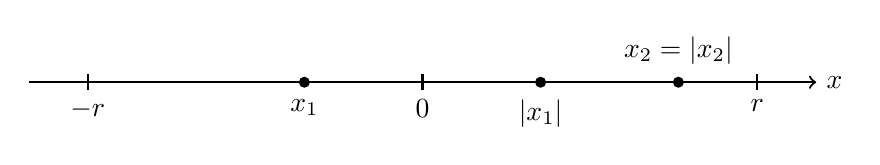
\begin{tikzpicture}[x=1cm, y=1cm]

  % The number line (axis)
  \draw[->, thick] (-5,0) -- (5,0) node[right] {\(x\)};
  \draw[thick] (0,0.1) -- (0,-0.1);
  \draw[thick] (-4.25,0.1) -- (-4.25,-0.1);
  \draw[thick] (4.25,0.1) -- (4.25,-0.1);

  % The actual points
  \fill (-1.5,0) circle (2pt);
  \fill (1.5,0) circle (2pt);
  \fill (3.25,0) circle (2pt);

  % Labels for r and -r
  \node[below, font=\normalsize] at (-4.25,-0.1) {\(-r\)};
  \node[below, font=\normalsize] at (-1.5,-0.1) {\(x_1\)};
  \node[below, font=\normalsize] at (0,-0.1) {\(0\)};
  \node[below, font=\normalsize] at (1.5,-0.1) {\(\lvert x_1 \rvert\)};
  \node[above, font=\normalsize] at (3.25,0.1) {\(x_2 = \lvert x_2 \rvert\)};
  \node[below, font=\normalsize] at (4.25,-0.1) {\(r\)};

\end{tikzpicture}
\end{document}
